\documentclass[12pt]{article}

\usepackage[ngerman]{babel}
\usepackage{hyperref}
\usepackage{geometry}
\usepackage{setspace}
\usepackage{helvet}
\usepackage{graphicx}

\geometry{
	a4paper,
	total={170mm,257mm},
	left=35mm,
	right=25mm,
	top=25mm,
	bottom=20mm
}


\renewcommand{\familydefault}{\sfdefault} % Setzt die Standardschriftart auf Helvetica (Äquibvalent zu Arial)

\linespread{1.5}


\renewcommand{\thefootnote}{\Roman{footnote}}

\begin{document}
	\pagenumbering{gobble}
	
	\title{Vergleich der Visualisierungsmöglichkeiten in Qlik und Python am Beispiel Human Development}
	\author{Philippe Denig, Jakob Dietrich, Luis Rastetter}
	\date{\today}
	
	\maketitle
	
	\newpage
	
	\tableofcontents
	
	\newpage
	
	
	\pagenumbering{arabic}
	\section{Einleitung} % Fomalien doppelchecken, falls notwendig (Umfang einhalten) anpassen
	
	% ChatGPT Quelle oder KI-Prüfung
	
	% Wieso braucht man DV, unterschiedliche Anwedungsszenarien brauchen unterschiedliche Tools, grober Überblick über das Vorgehen
	% einordbar deutsches Wort?
	Datenvisualisierung ist ein wichtiger Bestandteil der modernen Datenanalyse. Visualisierungen ermöglichen es, komplexe Informationen effektiv darzustellen und zu kommunizieren, sodass der Empfänger diese schnell erfassen kann. Dadurch spielt Datenvisualisierung in der Wirtschaft und Wissenschaft, aber auch im Privatleben eine entscheidende Rolle, um Erkenntnisse zu gewinnen und Zusammenhänge zu verstehen. Insbesondere im Geschäftsumfeld können Visualisierungen dazu beitragen, einen Überblick zu schaffen und so bei Entscheidungsfindungen zu unterstützen.
	
	Aufgrund der Bedeutung der Datenvisualisierung gibt es eine Vielzahl von Tools und Technologien, die mit unterschiedlichen Ansätzen und Funktionen versuchen bestmögliche Ergebnisse zu liefern. In dieser Arbeit wird sich mit der Programmiersprache Python im Datenvisualisierungskontext und der Business Intelligence (BI) Plattform Qlik beschäftigt. Dabei soll gezeigt werden, welches Tool sich besser für verschiedene Anwendungszwecke eignet.
	
	Um einen fundierten Vergleich zu ermöglichen, werden erst beide Tools kurz vorgestellt. Anschließend erfolgt eine systematische Evaluierung anhand verschiedener Aspekte, die sich an den einzelnen Schritten des CRISP-DM Verfahrens orientieren. Das CRISP-DM Verfahren besteht aus den Phasen Business Understanding, Data Understanding, Data Preparation, Modeling, Evaluation und Deployment. Es wird sich jedoch überwiegend auf die Phasen konzentriert, die durch die Tools beeinflusst werden: Data Understanding, Data Preparation und Modeling. Business Understanding, Evaluation und Deployment betreffen primär strategische Aspekte und werden daher nicht näher betrachtet. Um einen konkreten Anwendungsfall zu illustrieren, wird das Thema Human Development als Beispiel herangezogen. Dadurch wird ein realer Kontext geboten, in dem die Wirksamkeit der Tools bei der Analyse komplexer sozialer und wirtschaftlicher Daten bewertet werden kann. Darüber hinaus wird eine zusätzliche Kategorie Sonstiges eingeführt, die sich mit anderen, nicht in den CRISP-DM Prozess einzuordnenden Aspekten wie Kostenstruktur oder Dokumentation und Support beschäftigt. Dadurch wird eine umfassendere Einschätzung in dem Gesamtkontext der Data Science und BI Aktivitäten eines Unternehmens ermöglicht.
	
	Das Ziel ist es, ein tiefgreifendes Verständnis für die Stärken und Schwächen von Python und Qlik im Rahmen der praxisrelevanten Abschnitte des CRISP-DM Verfahrens zu erlangen. Auf Basis dieser methodischen Herangehensweise kann in Zukunft die Entscheidung des am besten für einen spezifischen Anwendungsfall geeigneten Visualisierungstools einfacher getroffen werden.
	
	\subsection{Was ist Qlik}
	Qlik ist eine der führenden Plattformen im Bereich der BI und wurde speziell für interaktive Datenanalyse und Datenvisualisierung konzipiert. Das Qlik Universum umfasst eine breite Produktpalette, durch die eine umfassende BI-Lösung zur datengetriebenen Entscheidungsunterstützung für Unternehmen verschiedener Größen und Branchen geboten wird. Im Zentrum stehen die beiden Datenvisualisierungs- und Datenanalyse-Tools Qlik View und Qlik Sense. Diese werden durch weitere Anwendungen wie z.B. Qlik Data für Datenmanagement unterstützt. Qlik View dient primär der Analytik und ist auf die Entwicklung von individuellen Anwendungen für die Datenanalyse ausgerichtet. Es ermöglicht Benutzern, komplexe Daten aus verschiedenen Quellen zu kombinieren, zu transformieren und zu visualisieren, um Einblicke zu gewinnen und fundierte Entscheidungen zu treffen. Qlik Sense wurde hingegen entwickelt, um eine breitere Benutzerbasis anzusprechen und bietet eine benutzerfreundliche, self-service-orientierte Plattform für die Datenvisualisierung und -analyse.
	
	In dieser Arbeit werden die Qlik Cloud Services in der "Qlik Sense Business - International Version"  betrachtet, da diese Version einen 30-tägigen Testzeitraum anbietet, mit dem unverbindlich und kostenlos ein umfassender Einblick in die Plattform gegeben wird. Außerdem bietet Qlik Sense im Vergleich zu Qlik View ein flexibleres Arbeitsumfeld und eine simplere Bedienung und steht somit mehr für moderne BI-Tools und grenzt sich weiter von Python ab.
	
	\subsection{Was ist Python}
	Python ist eine der am weitesten verbreiteten Programmiersprachen und spielt eine zentrale Rolle im Feld der Datenvisualisierung. Dank vieler starker Bibliotheken in diesem Bereich wie z.B. Matplotlib, Seaborn und Plotly bietet Python eine schier endlose Bandbreite an Möglichkeiten. Matplotlib bietet eine solide Grundlage für Diagramme und Grafiken, Seaborn hingegen stellt einen mehr auf Statistik basierneden Ansatz dar und mit Plotly können die Darstellungen weiter verfeinert werden, indem z.B. interaktive Elemente hinzugefügt werden. Außerhalb des tatsächlichen Visualisierungsprozesses kommen noch weitere Datenverarbeitungswerkzeuge wie Numpy und Pandas hinzu. Außerdem hat Python eine sehr große Community und es existieren zahlreiche kostenlose Lernunterstützungen.
	Insgesamt ist Python eine flexible Basis und in Kombination mit den entsprechenden Bibliotheken bietet Python breit gefächerte Möglichkeiten im Bereich der Datenvisualisierung.
	
	\subsection{Datensätze}
	Da der Toolvergleich am Beispiel Human Development durchgeführt wird, werden hier kurz die verwendeten Datensätze und deren Quellen vorgestellt.
	Human Development ist ein sehr breites Themengebiet, hier werden daher nur einzelne Aspekte wie Lebenserwartung, Geburtenrate und Todesfälle durch Naturkatastrophen betrachtet.
	
	Dazu werden insgesamt 10 Datensätze genutzt, 7 davon stammen von UNData. UNData ist eine Datensammlung der Vereinten Nationen über verschiedenste Themen, unter anderem Human Development. Die verwendeten Datensätze sind in ihrem Format daher sehr ähnlich und bestehen immer aus den Spalten Land, Jahr und dem Wert des jeweiligen Datensatzes. Somit liegt immer nur eine Datenspalte pro Datensatz vor, weshalb sieben Datensätze benötigt werden. Die Daten stammen primär von den einzelnen Unterorganisationen der UN wie beispielsweise der World Health Organisation (WHO) und sind somit als seriös einzustufen. Einer der übrigen drei Datensätze über Selbstmordraten stammt von der WHO direkt, da er nicht über UNData veröffentlicht wurde und ist somit ebenfalls als gesicherte Quelle zu betrachten. Die restlichen beiden Datensätze stammen von Kaggle, einem Webportal, auf dem Datensätze veröffentlicht werden können. Die ursprüngliche Quelle des Datensatzes über Naturkatastrophen liegt dabei bei der NASA und wurde größtenteils mit dem Satellitenprogramm Earth Observing System Data and Information System (EOSDIS) und dessen Vorgängern gesammelt. Grundsätzlich liefert dieser Datensatz also ebenfalls verlässliche Daten, es gilt aber zu beachten, dass die Daten zwar bis 1900 zurückreichen, aber bis 1970 insbesondere kleinere Naturkatastrophen fehlen. Der letzte Datensatz ist der World Happiness Report.
	aus dem Jahr 2021. Dieser bewertet das Glücksempfinden der Menschen verschiedener Länder und wird von einem internationalen Team aus Wissenschaftlern zusammengestellt, weshalb auch dieser eine seriöse Quelle darstellt. Es gilt allerdings zu beachten, dass der hier verwendete finale Wert des Glücksempfindens auf Basis vieler Faktoren berechnet wird und nur ein Teil der Bewertung auf Umfragen an den Bürgern der Länder basiert.
	
	Durch die Verwendung solch qualitativ hochwertiger und verlässlicher Datensätze wird sichergestellt, dass die zum Thema Human Development gewonnenen Erkenntnisse aussagekräftig sind und dass die Visualisierungen mit den beiden Tools in einer realistischen Situation getestet und bewertet werden können.
	\section{Vergleich zwischen Qlik und Python}
	
	\subsection{Einleitung Vergleich}
	Wie bereits in der Einleitung erwähnt, erfolgt der Vergleich vorwiegend anhand der relevanten Phasen des CRISP-DM Prozesses. In den einzelnen Phasen werden Python und Qlik auf Basis verschiedener für die jeweilige Phase relevanten Kriterien evaluiert und es wird ein Bezug zu dem Thema Human Development hergestellt, das insbesondere durch die große Anzahl an verschiedenen Datensätzen eine besondere Herausforderung darstellt. Im folgenden Vergleich wird davon ausgegangen, dass der Anwender Grundkenntnisse in der Programmierung besitzt, da andernfalls eine Verwendung von Python ohne vorherigen Lernprozess nicht infrage kommt. Python ist zwar im Vergleich zu anderen Programmiersprachen recht intuitiv, aber dennoch nicht ohne Programmierkenntnisse bedienbar. Die erforderlichen Programmierkenntnisse stellen einen Nachteil dar, auf diesen wird erneut im Fazit eingegangen.
	
	\subsection{Data Understanding}
	Im ersten Schritt des Toolvergleichs wird sich auf das Data Understanding fokussiert, bei welchem es darum geht, die Daten im entsprechenden Tool hinzuzufügen und eine umfassende Übersicht über die verfügbaren Datenquellen, deren Qualität, Struktur und potenzielle Einschränkungen zu gewinnen.

	In Qlik lassen sich neue Datensätze in Form von einzelnen Dateien schnell per Drag-and-Drop hinzufügen und es werden alle gängigen Dateiformate bis auf JSON unterstützt. Bei JSON Dateien ist eine Vorverarbeitung notwendig. Das Hinzufügen der Dateien in Python dauert bedeutend länger, da sie erst per Codezeile eingelesen werden müssen und das Schreiben dieser einige Zeit braucht, dafür existieren keinerlei Einschränkungen bezüglich des Dateiformats.
	\begin{figure}[h]
		\centering
		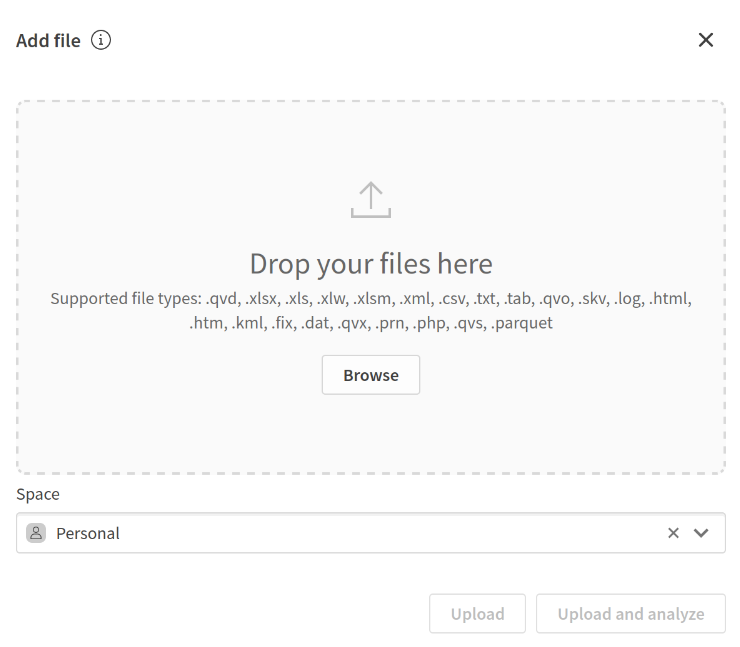
\includegraphics[width=0.5\textwidth]{dragndrop}
		\caption{Drag-and-Drop}
	\end{figure}
	
	Der Prozess des Daten Hinzufügens in Qlik ist intuitiv und gut beschrieben, sodass bei der ersten Nutzung alles ohne Probleme funktioniert hat. Auch große Datensätze stellen kein Problem dar. Laut Qlik liegt die maximale Dateigröße bei 100 Gigabyte. Die Geschwindigkeit des Uploads hängt von der Uploadgeschwindigkeit des Users ab, da die hier genutzte Qlik Version mit einer Cloud arbeitet. Python kann sowohl lokal, als auch in einer Cloud verwendet werden. Bei lokaler Nutzung gibt es keine Verzögerungen durch den Upload, bei Nutzung einer Cloud hängt es ebenfalls von der Uploadgeschwindigkeit des Nutzers ab.
	In Python ist eine Nutzung von APIs mit entsprechenden Bibliotheken wie z.B. Request einfach möglich.
	Auch in Qlik können APIs verwendet werden, aber die Anzahl der APIs ist begrenzt.
	
	In dem hier verwendeten Beispiel Human Development wird eine größere Anzahl an Datensätzen benötigt. Qlik bietet eine gute Übersicht darüber, welche Datensätze hochgeladen sind. Die Datensätze lassen sich in Raster- und Listenansicht anzeigen und nach Kriterien wie als letztes genutzt sortieren und es können Favoriten festgelegt werden. In Python kann durch eine übersichtliche Ordnerstruktur in Kombination mit einer guten IDE der Überblick über die verschiedenen Dateien bewahrt werden.
	
	Der nächste wichtige Schritt des Data Understanding ist die Datenexploration. Das Tool sollte dem Nutzer die Möglichkeit bieten, einen groben Überblick über den Datensatz zu bekommen, speziell das Erkennen von NaN-Werte spielt hier eine große Rolle.
	
	In Python lässt sich Datenexploration insbesondere mit Pandas gut durchführen. Durch die Nutzung eines Panda Dataframes werden dem Nutzer viele Befehle wie head(), info() und describe() zur Verfügung gestellt. Mit diesen lässt sich ein guter Überblick über die Struktur des Datensatzes erhalten. Zudem gibt es die Funktion isna(), mit der NaN-Werte identifiziert werden können.	
	\begin{figure}[h]
		\centering
		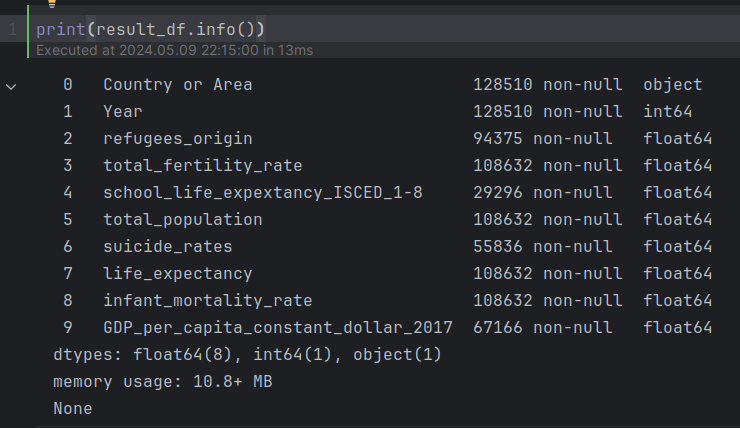
\includegraphics[width=0.5\textwidth]{info()}
		\caption{Drag-and-Drop}
	\end{figure}
	In Qlik kann über die allgemeine Struktur des Datensatzes in dem Reiter Überblick eine gute Übersicht erstellt werden. Für weitere Details kann in den Reiter Felder gewechselt werden. In diesem sind Informationen über die einzelnen Spalten eines Datensatzes zu finden und es werden Visualisierungen zur Verteilung der Werte angezeigt. Zudem ist hier ein Einblick der ersten 10 Zeilen in Tabellenform, sowie eine Auflistung der einzelnen Spalten inklusive Datentyp zu finden.
	
	Bisher liegen in Qlik die Daten nur als einzelne in die Cloud hochgeladene Dateien vor, mit ihnen kann aber noch nichts bis auf die Datenexploration der einzelnen Datensätze durchgeführt werden. Um die Daten weiter zu verarbeiten, muss eine App (ein Arbeitsdokument, das eine analytische Anwendung darstellt) erstellt werden und die Daten müssen hinzugefügt werden. Das Hinzufügen der Daten geht einfach, der Benutzer kann aus den Daten, die er in Qlik hochgeladen hat, auswählen, welche er der App hinzufügen möchte. Es ist auch möglich, nur einzelne Spalten aus Datensätzen auszuwählen. Dieser Prozess hat in der Basisversion ein Limit von 1260 Megabyte und dauert bei größeren Datensätzen bis hin zu einigen Minuten.
	Nach dem Datenupload werden sofort, ohne dass weitere Aktionen des Benutzers erforderlich sind, Vorschläge unterbreitet, anhand welcher Spalten sich die einzelnen Datensätze miteinander verknüpfen lassen. Anschließend können im Datenmanager die einzelnen Datensätze per Drag-and-Drop ent- und verknüpft werden.
	\begin{figure}[h]
		\centering
		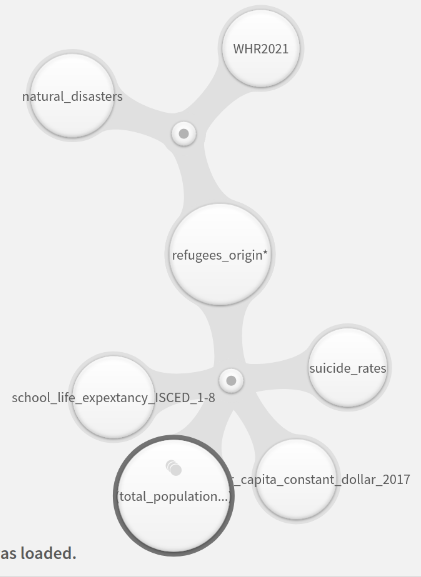
\includegraphics[width=0.5\textwidth]{connect}
		\caption{Drag-and-Drop Verknüfung}
	\end{figure}
	Die zusammengehörenden Spalten werden automatisch festgestellt. Falls dies nicht möglich ist, kann manuell gewählt werden, welche Spalten verknüpft werden sollen.
	Es ist in Qlik auf diesem Weg nicht möglich, einzelne Datensätze über zwei Mountpoints miteinander zu verknüpfen, was am Beispiel der Human Development Datensätze erforderlich gewesen wäre. Stattdessen kann diese Vernüpfung nur über Skripte in Qlik erreicht werden, was immer noch den Vorteil gegenüber einer Vorbearbeitung in Python hat, dass alles in einer Anwendung ablaufen kann und keine Daten übertragen werden müssen.
	Außerdem können hier Datensätze in zwei Teile aufgetrennt werden.
	Im Datenmanager existiert neben der Verknüfungsperspektive die Tabellenperspektive. Hier lässt sich nach einem einzelnen Wert, wie z.B. einem NaN-Wert suchen.
	Zur besseren Visualisierung der Verknüpfungen kann auch in den Datenmodell-Viewer gewechselt werden, hier sind die einzelnen Datensätze in Tabellenform mit Verknüpfungen zwischen den einzelnen Spalten dargestellt.
	\begin{figure}[h]
		\centering
		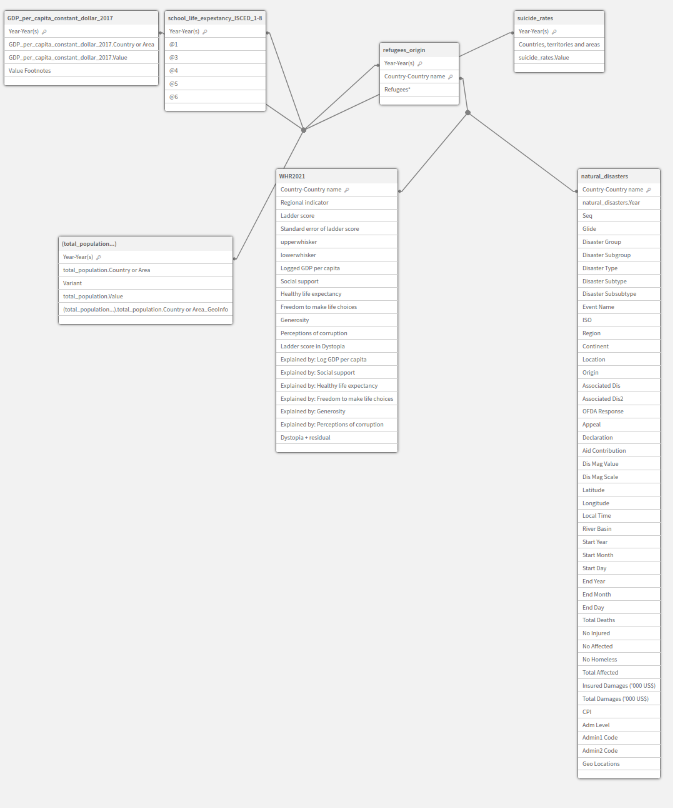
\includegraphics[width=0.5\textwidth]{table_viewer}
		\caption{Datenmodell-Viewer}
	\end{figure}
	Nach jeder Änderung im Datenmanager müssen die Daten erneut wenige Sekunden geladen werden, bevor weiter mit ihnen gearbeitet werden kann.
	Nach Verlassen des Datenmanagers ist es möglich, mit dem Insight Advisor zu den einzelnen Spalten verschiedene Visualisierungen zu erstellen, zusätzlich ist das auch durch eine Beschreibung mit natürlicher Sprache möglich. In Python würden solche Visualisierungen zur Datenexploration vergleichsweise lange dauern.
	\begin{figure}[h]
		\centering
		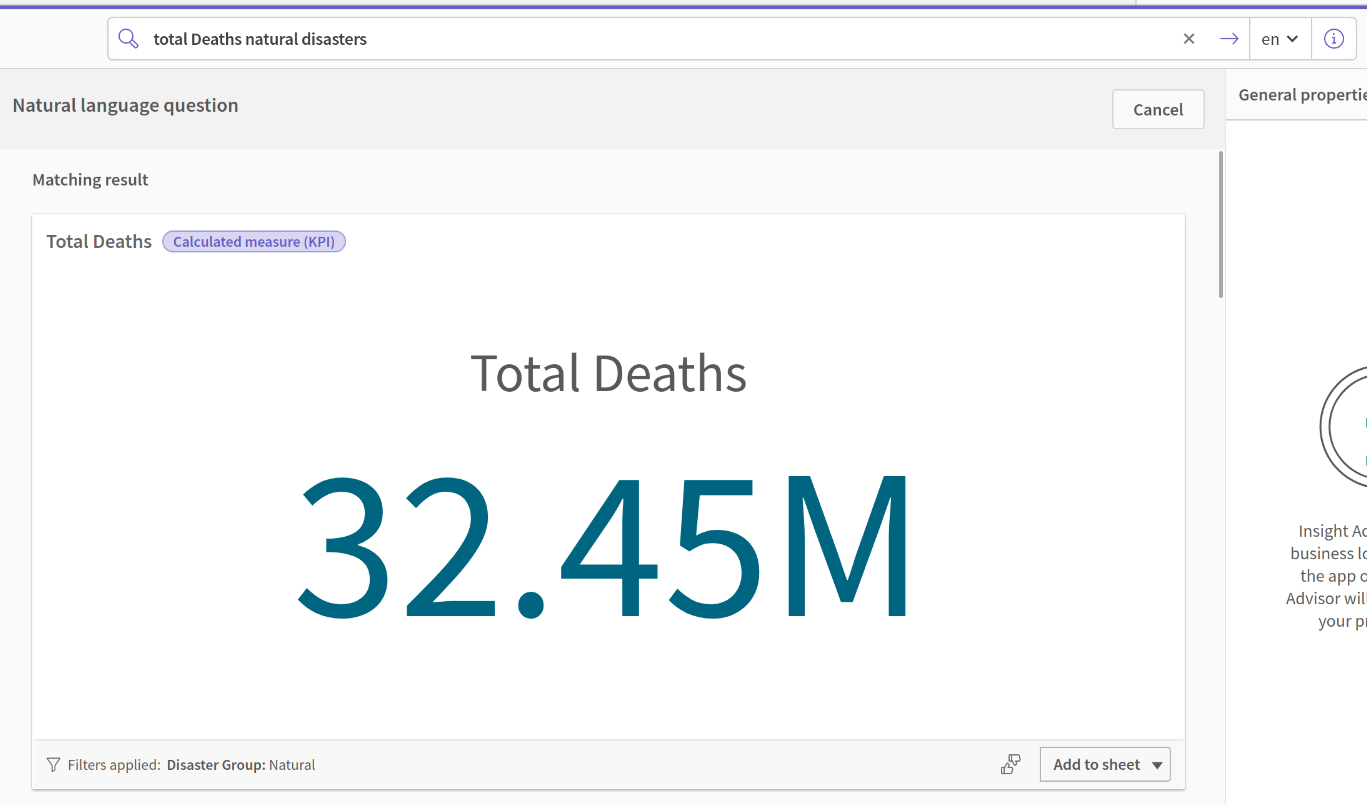
\includegraphics[width=0.5\textwidth]{bsp_ask}
		\caption{Insight Advisor - natürliche Sprache}
	\end{figure}
	
	Somit stellt Qlik eine ähnliche Bandbreite an Data Understanding Funktionen wie Python zur Verfügung, während die meisten Prozesse deutlich schneller und effizienter ablaufen. Es treten primär Probleme bei der Verarbeitung von JSON Dateien und bei sehr großen Dateien über einem Gigabyte auf.
	
	\subsection{Data Preparation}
	In der Data Preparation geht es darum, die Daten für die Analyse vorzubereiten, indem sie gereinigt, transformiert und in das richtige Datenformat gebracht werden, um sicherzustellen, dass sie für den Modellierungsschritt geeignet sind.
	Ein wichtiger Schritt dazu besteht darin, NaN-Werte zu entfernen und Zeilen und Spalten zu editieren. In Python kann das mit den entsprechenden Befehlen wie dropna() oder fillna() der Pandas Bibliothek ohne großen Zeitaufwand umgesetzt werden.
	Qlik bietet diese Funktionen im Tabelleneditor.
	
	\begin{figure}[h]
		\centering
		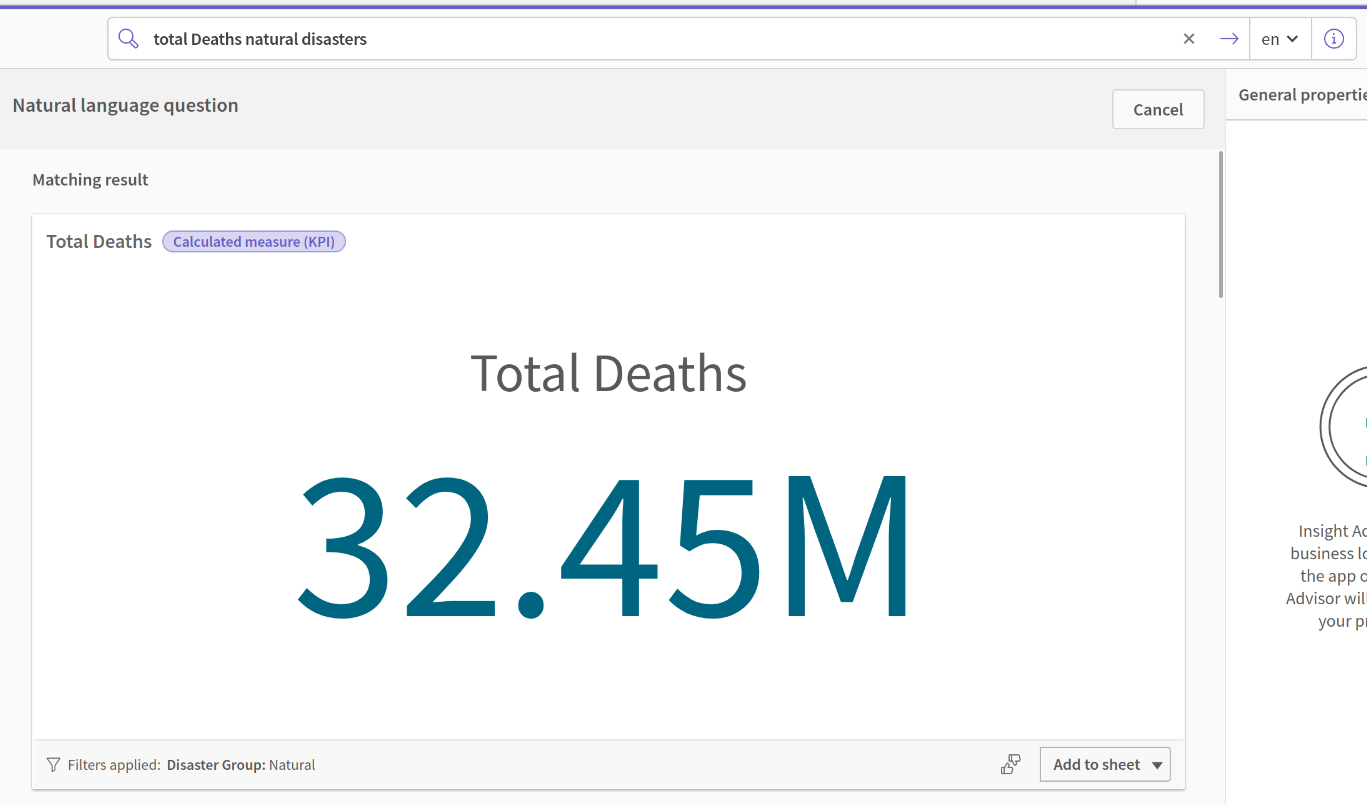
\includegraphics[width=0.5\textwidth]{bsp_ask}
		\caption{Insight Advisor - natürliche Sprache}
	\end{figure}
	\begin{figure}[h]
		\centering
		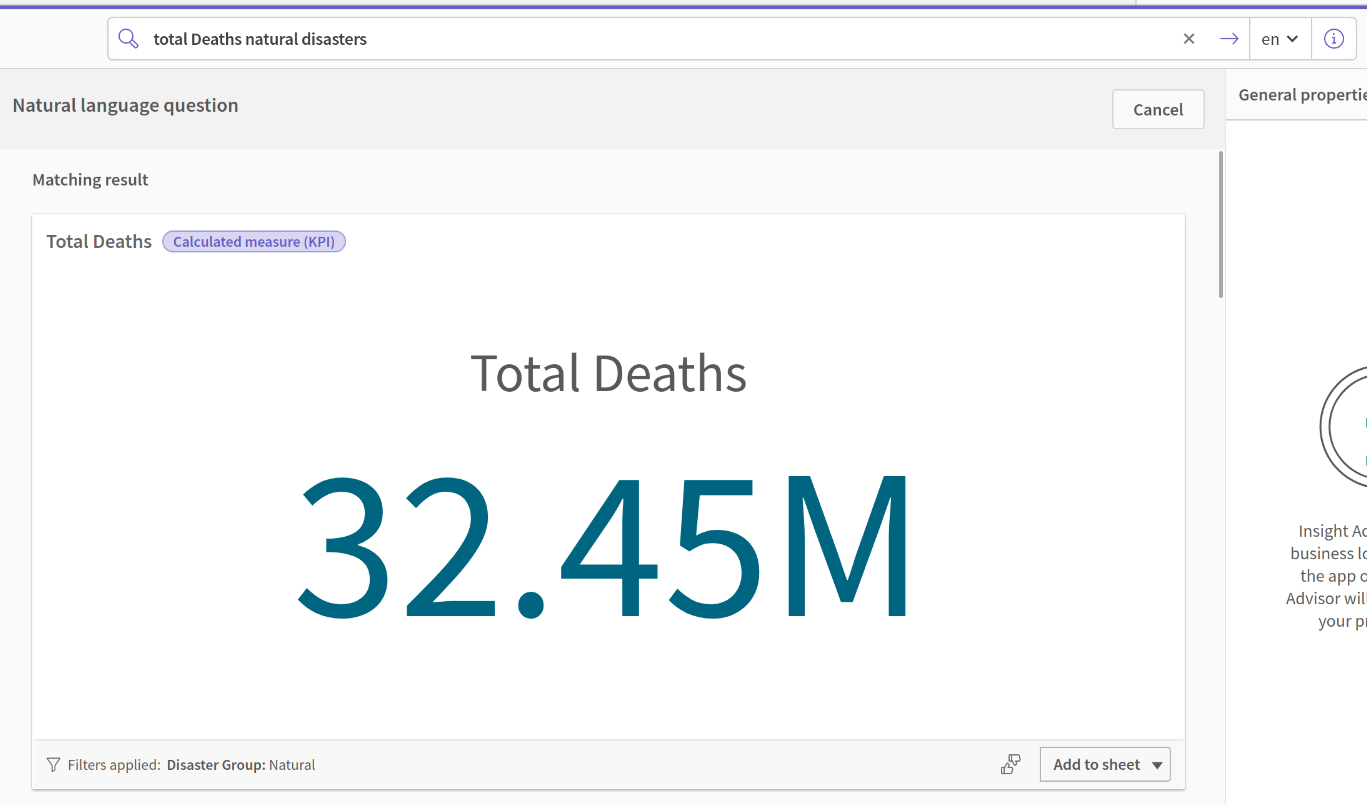
\includegraphics[width=0.5\textwidth]{bsp_ask}
		\caption{Insight Advisor - natürliche Sprache}
	\end{figure}
	
	
	Strukturänderungen im Datensatz wie z.B. Aggregation und Disaggregation sind auch in beiden Tools möglich, in Python z.B. mit groupby() mit entsprechenden Parametern, in Qlik gibt es die Funktionen Sum(), Avg(), Count(), Min() und Max().
	Datenverknüpfungen in Qlik wurden im letzten Abschnitt  ausreichend beschrieben, in Python ist das mit der  merge() Funktion ebenfalls möglich.
	Datentypänderungen sind in Qlik im Datenmanager möglich, in Python sind sie mit der Funktion astype() umsetzbar.
	Insgesamt unterscheiden sich Qlik und Python im Bereich Data Preparation kaum, Qlik ist zwar schneller, aber die meisten Python Befehle sind nur wenigen Zeichen lang und somit auch schnell ausgeschrieben und der Zeitunterschied ist sehr gering. Qlik bietet alle grundlegenden Funktionen, für spezialisiertere Anwendungsfälle stößt man ohne Anwendung von Skripten allerdings schnell an Grenzen. Dementsprechend ist Qlik im Bereich Data Preparation eher für die Anwendung auf qualitativ hochwertigeren Daten geeignet und kann dort einfach Strukturänderungen und Ähnliches durchführen.
	
	
	\subsection{Modeling}
	Im Modeling-Schritt werden die vorbereiteten Daten verwendet, um Visualisierungsmodelle zu erstellen. Ziel ist es, visuelle Darstellungen und Interaktionsmöglichkeiten zu entwickeln, die es ermöglichen, Muster, Trends und Beziehungen in den Daten zu erkennen und zu kommunizieren.
	
	Zur finalen Visualisierung von Daten in Qlik muss zunächst ein Sheet erstellt werden, dann stehen verschiedene Diagrammarten zur Verfügung, zu denen dann die entsprechenden Daten zugeordnet werden.
	In Python sind grundsätzlich alle Diagrammarten möglich. Die Auswahl in Qlik ist etwas begrenzter, aber die grundlegenden Diagramme wie Balken-, Linien-, Kreis- und auch etwas komplexere Diagramme wie Heatmaps, Histogramme und eine Weltkarte sind verfügbar. 
	\begin{figure}[h]
		\centering
		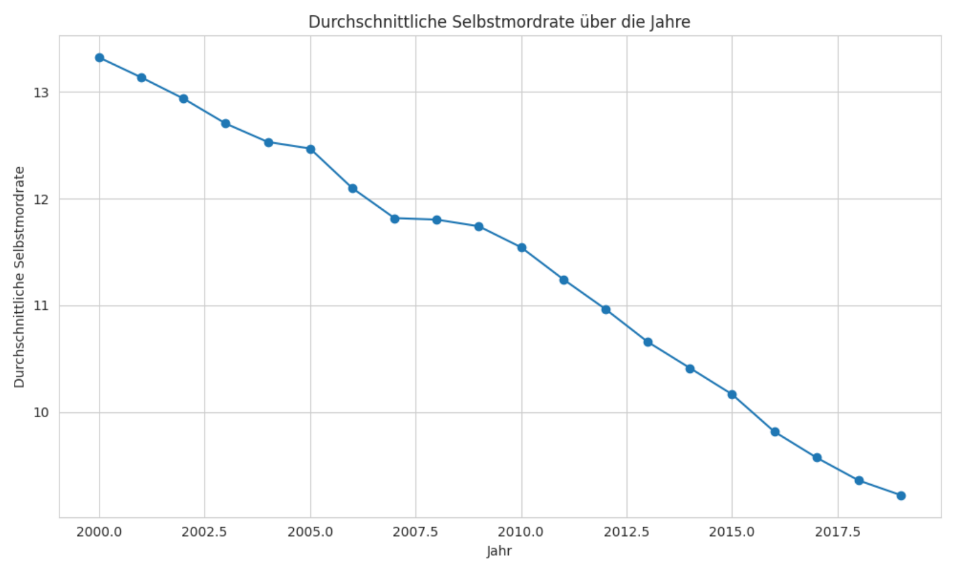
\includegraphics[width=0.5\textwidth]{easy_linechart}
		\caption{durchschnittliche Selbstmordraten als Beispiel einer einfachen Visualisierung in Qlik}
	\end{figure}
	
	Es fehlen z.B. Gantt-Charts zur Visualisierung von Projektphasen oder Violin Plots.
	Im Bereich Human Development spielen Geovisualisierungen eine wichtige Rolle. Qlik bietet eine Weltkarte zur Visualisierung, manuell muss nur die entsprechende Zeile mit Strings die Länder, Regionen oder Städte beschreiben oder Geokodierungsinformationen, wie Längen- und Breitengrade der Weltkarte zugeordnet werden, dann wird automatisch eine entsprechende Karte erstellt, durch die Zoomfunktion ist es auch möglich kleinere Regionen detailliert darzustellen. In Python sind Geovisualisierung mit den Bibliotheken Matplotlib und Plotly ebenfalls möglich, indem nur die entsprechende Spalte zugeordnet wird und die Zuordnung der Länder auf der Karte erfolgt automatisch. In Python sind insbesondere die Gestaltungsmöglichkeiten weniger begrenzt als bei Qlik.
	\begin{figure}[h]
		\centering
		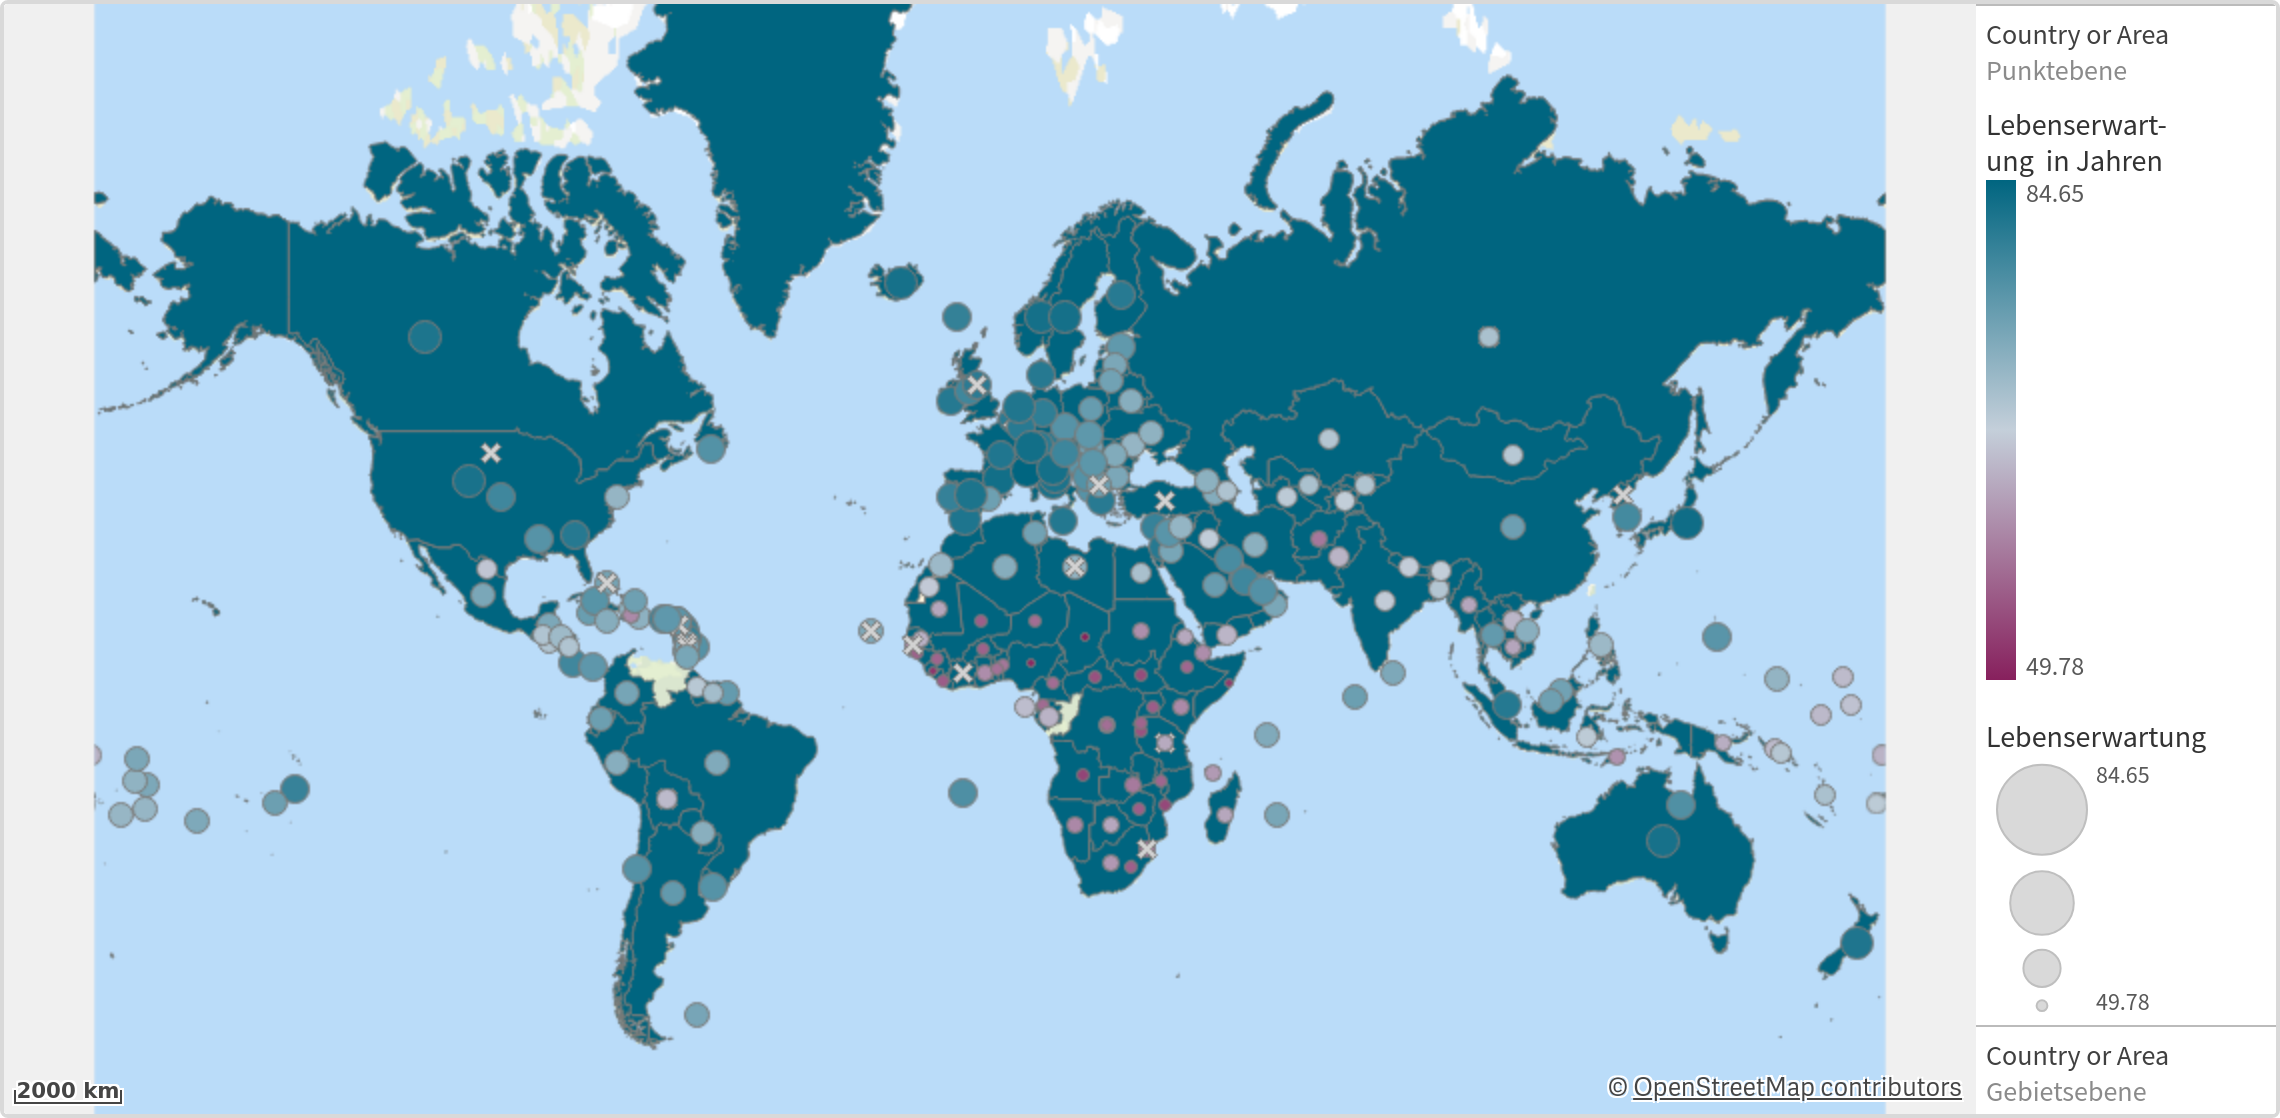
\includegraphics[width=0.5\textwidth]{life_exp_qlik}
		\caption{Lebenserwartung 2020 visualisiert mit Qlik}
	\end{figure}
	\begin{figure}[h]
		\centering
		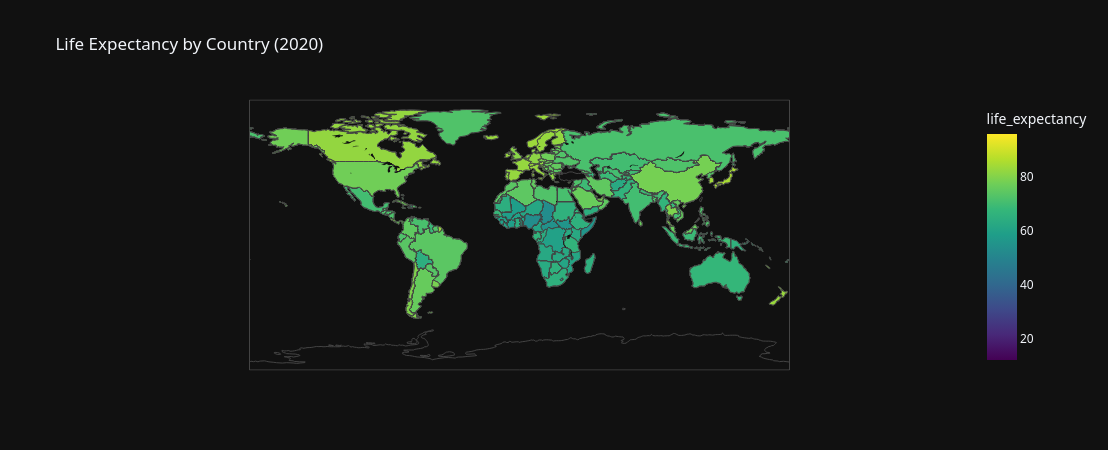
\includegraphics[width=0.5\textwidth]{life_exp_python}
		\caption{Lebenserwartung 2020 visualisiert mit Python}
	\end{figure}
	
	Hier fällt z.B. auf, dass in Python die gesamten Länder entsprechend der Skala eingefärbt werden können.
	Insbesondere die farblichen Gestaltungsmöglichkeiten sind in Python deutlich ausgeprägter, bei anderen Gestaltungen wie z.B. Achsenbeschriftungen bietet Qlik alle notwendigen Features. Auch die Qualität ist mit beiden Tools auf einem hohen Niveau, es treten keine unscharfen Stellen oder Überlappungen auf. Der allgemeine Prozess der Erstellung einer Visualisierung ist in Qlik schnell und intuitiv durchzuführen, zuerst wird der Diagrammtyp gewählt, dann den Achsen eine Spalte aus den Tabellen zuweisen und dann ist die Visualisierung schon fertig. In Python sind Visualisierungen ein deutlich größerer Zeitaufwand, da auch bei sehr simplen Visualisierungen die Zuweisungen immer getippt werden müssen. Dadurch wird grundsätzlich mehr Zeit beansprucht, auch wenn der Programmierer alle notwendigen Befehle kennt, was insbesondere bei einer größeren Bandbreite an Visualisierungen nicht unbedingt der Fall ist. Falls die für eine Visualisierung benötigten Daten nicht direkt vorliegen, sondern erst noch aus anderen Spalten berechnet werden müssen, bietet Qlik die Möglichkeit eine neue Spalte aus bestehenden mit einer frei wählbaren Formel zu berechnen. Die Auswahl an Rechenoperationen für einen solchen Anwendungsfall begrenzter als in Python, es existieren auch Funktionen um Strings zusammenzusetzen. Und falls die direkt verfügbaren Funktionen nicht ausreichen, gibt es durch Skripts noch weitaus mehr Optionen.
	Die Echtzeitdaten, die über eine API integrierbar sind, lassen sich auch in Echtzeit visualisieren, die Visualisierungen im Tool werden also verändert, wenn neue Daten hinzugefügt werde. Dadurch ist es in Qlik auch möglich, Dashboards zu erstellen, die in Echtzeit bestimmte Daten anzeigen können. Um ein Dashboard zu erstellen werden natürlich einige Grafiken, Steuerlemente und Weiteres benötigt und die Erstellung benötigt einige Zeit, aber es geht immer noch bedeutend schneller als in Python, auch wenn natürlich etwas an Funktionen verloren geht.
	Die Visualisierungen in Qlik laden auch schnell unter der Verwendung von sehr großen Datensätzen und stehen Python um nichts nach.
	In Punkten Statistik kann Qlik dann nicht mehr mit Python mithalten. Qlik bietet einige Basisfunktionen wie Mittelwertberechnungen und Medianberechnungen, aber für fortgeschrittenere statistische Berechnungen oder maschinelles Lernen bietet es keine Funktionen. Das ist aber auch nicht der Anwendungszweck einer BI Plattform. In Python ist diese Verwendung mit Bibliotheken wie SciPy möglich.
	Zusammenfassend bietet Qlik alle grundlegendes Funktionen die für einfache und etwas fortgeschrittenere Visualisierungen benötigt werden, aber wenn es an speziellere Visualisierungen oder eher mathematische Methoden geht, stellt Qlik keine entsprechenden Features bereit.
	
	\subsection{Sonstiges}
	Zusätzlich zu den drei Hauptphasen des Toolvergleichs gibt es einen Sonstiges-Schritt, der sich mit anderen wichtigen Aspekten wie Kosten, Benutzerfreundlichkeit, Support und anderen nicht direkt im CRISP-DM Prozess enthaltenen Faktoren befasst.
	Insbesondere ohne vorherige Programmiererfahrung ist der Anfang in Python schwer. Aber durch eine Vielzahl von Büchern, Videos und anderen unterstützenden Lernmaterialien ist es möglich Python in einem angemessenen Rahmen zu erlernen. Zu Qlik gibt es deutlich weniger Lernmaterialien, aber ein dennoch vollkommen ausreichender Umfang. Unter anderem stellt Qlik selbst eine Online Lernplattform zur Verfügung. Ähnlich verhält es sich mit der Dokumentation, Foren und Communitys und KI. Bei allem gibt es mehr bezüglich Python, aber auch bei Qlik sind die Informationen vollkommen ausreichend. Stabilitätsproblem sind bei keinem der beiden Tools aufgefallen. Kollaboratives Arbeiten wird immer wichtiger, speziell in den Bereichen Datenanalyse und BI. In Python findet die Zusammenarbeit für gewöhnlich über Versionskontrollsysteme wie z.B. git oder Cloudplattformen wie Google Colab statt. Qlik bietet für den Unternehmensgebrauch eine integrierte Lösung mit einer Vielzahl von Kollaborationsmöglichkeiten wie z.B. der Storytelling-Funktion, mit der durch Datenpräsentationen kommuniziert werden kann.
	In Python können Daten in wenigen Zeilen Code in einer Vielzahl von Dateiformaten exportiert werden, Qlik bietet weniger Optionen, aber die wichtigsten wie csv, xml für Daten und pdf und png für Grafiken sind verfügbar. Python ist grundsätzlich kostenlos und Open Source, einige spezielle Bibliotheken und wenn notwendig Cloud Plattformen können aber Kosten verursachen. Die Preisgestaltung bei Qlik ist etwas komplizierter, es gibt grundsätzlich drei verschiedene Pakete mit unterschiedlichen Features % Bild
	
	 Vollbenutzer sind Benutzer, die vollen Zugriff auf alle Funktionen haben, Basisbenutzer können nur mit den Apps interagieren und sie sich anschauen.
	Die Preisgestaltung für zusätzliche Vollbenutzer und Basisnutzer ist leider nicht zu finden, es gibt nur eine Preistabelle für weitere andere Nutzungsarten.
	% Bild
	\section{SWOT Analyse}
	
	\subsection{Python}
	
	\subsubsection{Data Scientist}
	
	Als Data Scientist erhält man mit Python ein Tool, das sehr flexibel im Umgang mit Daten
	ist. Zudem ist es kostenlos und erhält diverse Möglichkeiten zur Visualisierung von
	Daten, womit die einzelnen Schritte des CRISP-DM Prozesses problemlos durchlaufen
	werden können.
	Weiter bieten die umfangreichen Bibliotheken und ausführlichen Dokumentationen
	viele Optionen zur Erweiterung und Implementierung neuer Features. Somit ist Python
	vielseitig einsetzbar und dient auch mit dem Einsatz von künstlicher Intelligenz als
	Universalwerkzeug.
	Außerdem bietet der Einsatz der Programmiersprache den Vorteil, dass bereits erlernte
	Kenntnisse nicht verlernt werden.
	Dennoch gibt es immer auch irgendwelche Nachteile oder mögliche Gefahren.
	So ist Python, wie im vorherigen Toolvergleich bereits erwähnt, nicht immer sehr
	übersichtlich und erfordert auch gute Programmierkenntnisse, damit adäquate
	Ergebnisse erzeugt werden können. Besitzt man diese nicht, wird es schwer geeignete
	Visualisierung zu entwerfen.
	Weiter sind im Umgang mit dem Datensatz zwar keine größeren Leistungsprobleme
	aufgetreten, dennoch gibt es andere Programmiersprachen, die etwas schneller
	arbeiten. Erahnen lassen konnte sich das anhand der Erstellung des Pair-Plots, da
	hierbei schon ein wenig mehr Zeit verstrichen ist, bis die Visualisierung sichtbar wurde.
	Auch ist der zu betreibende Aufwand für gute Modellierungen durchaus als Schwäche
	anzuerkennen, was natürlich auch die Gefahr bringt, dass mit der Zeit Konkurrenz durch
	spezialisierte Software auf dem Markt entsteht, in welcher dieser Aufwand verringert wird.
	\begin{figure}[h]
		\centering
		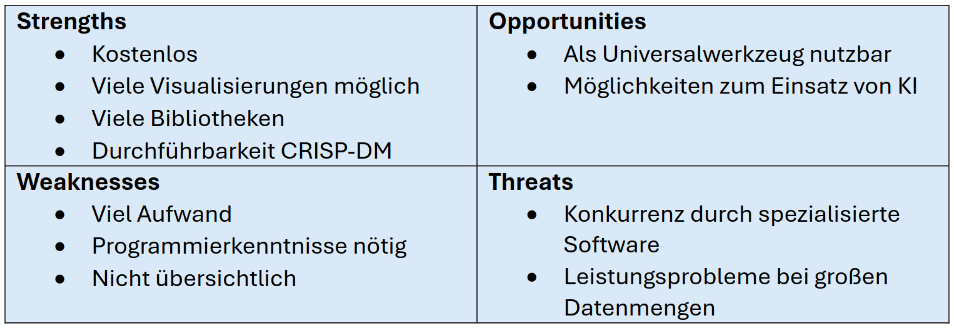
\includegraphics[width=0.5\textwidth]{SWOT1}
		\caption{SWOT Analyse Python Data Scientist}
	\end{figure}
	
	\subsubsection{Betrieblicher Entscheider}
	
	Als betrieblicher Entscheider hat man differenzierte Präferenzen als ein Data Scientist,
	der jeden Tag mit diversen Daten arbeitet. So muss man auch Geschäftsdaten in einem
	Dashboard präsentieren, um später damit mögliche Geschäftsentscheidungen
	begründen zu können. Dementsprechend ist es hierfür notwendig, eine zweite SWOT-
	Analyse zu konfigurieren.
	Für betriebliche Entscheider, für die nicht die besten Erfahrungen im Umgang mit Python
	zu erwarten sind, bietet die Programmiersprache vor allem Stärken, indem sie sehr
	umfangreiche Bibliotheken und auch viele unterstützende Dokumentationen besitzt.
	Damit kann vielen Unerfahrenen geholfen werden, geeignete Modellierungen zu
	konzipieren. Dies eröffnet zudem die Möglichkeit, spätere Dashboards in Hinsicht auf
	jede Komponente individuell anzupassen, weil die Bibliotheken nahezu unbegrenzt sind
	und gut erklärt werden.
	Ferner kann Python auch in andere unternehmensinterne Software integriert werden,
	sodass es auch abseits der Daten Visualisierung vielfach zum Einsatz kommen kann.
	Allerdings stehen auf der gegenüberliegenden Seite auch einige Schwachstellen, welche
	Python in Bezug auf die Nutzung durch einen betrieblichen Entscheider offenbart.
	So gibt es zum Beispiel keine Standardisierung von Dashboards innerhalb des Tools. Vor
	allem bei mangelhaften Programmierkenntnissen, kann es in diesem Fall schwer
	werden geeignete und anschauliche Dashboards für die Präsentation gegenüber Dritten
	zu erstellen. Diese fehlende Ästhetik birgt auch die Gefahr, dass dadurch eine gewisse
	Überzeugungskraft der Daten verloren geht und der hohe Aufwand mehr oder minder
	umsonst aufgebracht wird.
	Damit zeigt Python einige Nachteile für Unternehmer auf, die lediglich Daten
	präsentieren wollen, aber nicht das nötige Hintergrundwissen für die Benutzung des
	Tools mitbringen.
	\begin{figure}[h]
		\centering
		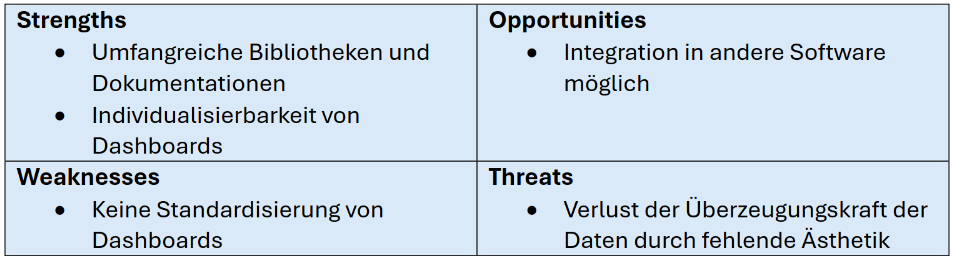
\includegraphics[width=0.5\textwidth]{SWOT2}
		\caption{SWOT Analyse Python Betrieblicher Entscheider}
	\end{figure}
	
	\subsection{Qlik}
	
	\subsubsection{Data Scientist}
	
	Um einem potenziellen Data Scientist verschiedene Optionen für den Einsatz eines
	Datenvisualisierungstools geben, soll nun noch eine SWOT-Analyse für das vorherige
	betrachtete Qlik präsentiert werden.
	Ansprechende Aspekte an Qlik für einen Data Scientist dürften definitiv darin beruhen,
	dass es wirklich benutzerfreundlich und übersichtlich ist. Selbst wenn zu spezifischen
	Aspekten Unklarheiten aufkommen sollten, können diese in den meisten Fällen mithilfe
	von Online-Tutorials und Dokumentationen beseitigt werden. Zu beinahe jedem Problem
	können Entscheidungsfindungen durch das Internet herangezogen werden.
	Was während der Test-Nutzung für die Tool-Analyse auch als Vorteil aufgetreten ist, ist
	die Leichtigkeit, mit welcher bei bereits gesäuberten Datensätzen verschiedene
	Modellierungen erstellt und auch die einzelnen Dimensionen und Ebenen verändert
	werden können.
	Dadurch entsteht die Möglichkeit ohne viel Aufwand schnell und direkt Visualisierungen
	zu erstellen und diese auch individuell anzupassen. Dies ist durchaus leichter
	vorzunehmen als in Python.
	Allerdings ist ein Data Scientist aber auch an einer möglichst großen Auswahl an
	Visualisierungselementen interessiert, da er möglichst breitgefächert auftreten will.
	Zwar konnten bezüglich des Themas Human Development alle Fragestellungen mit den
	vorhandenen Visualisierungsarten bearbeitet werden, dennoch können einige Modelle
	innerhalb des Tools vermisst werden. So sind beispielhaft der Violin-Plot, der Pair-Plot
	und auch die Korrelationsmatrix nicht nutzbar.
	Im Vergleich bietet Python durch die Erweiterbarkeit der vielen Bibliotheken eine
	deutlich größere Palette an Möglichkeit, sodass beim Einsatz von Qlik auf einige
	Grafiktypen verzichtet werden muss.
	Weiter ist für den Data Scientist aber auch die fehlende Möglichkeit für das Data
	Cleaning und die Data Preparation ein Nachteil, da Datenmengen, welche
	Inkonsistenzen beinhalten, somit weniger gut bearbeitet werden können. Dies führt
	folgendermaßen zu schlechteren Visualisierungen und dementsprechend auch einem
	geringeren Nutzwert für den Endanwender.
	Außerdem ist die kostenlose Test-Version von Qlik nur für 30 Tage gültig, wodurch die
	Gefahr besteht, dass längerfristige Projekte nur mit dem Einsatz dieses Tools und ohne
	den Einsatz von zusätzlichen Kosten nicht möglich sind. Für einen Data Scientist, der
	womöglich noch privat mit dem Tool arbeiten will, sind 30 US-Dollar pro Monat nämlich
	schon eine beträchtliche Summe.
	Zudem macht man sich durch den Kauf des Tools auch abhängig vom Verkäufer, indem
	man auf die neuesten Updates und Features warten muss, während diese womöglich in
	anderen Tools schon vorhanden sind.
	\begin{figure}[h]
		\centering
		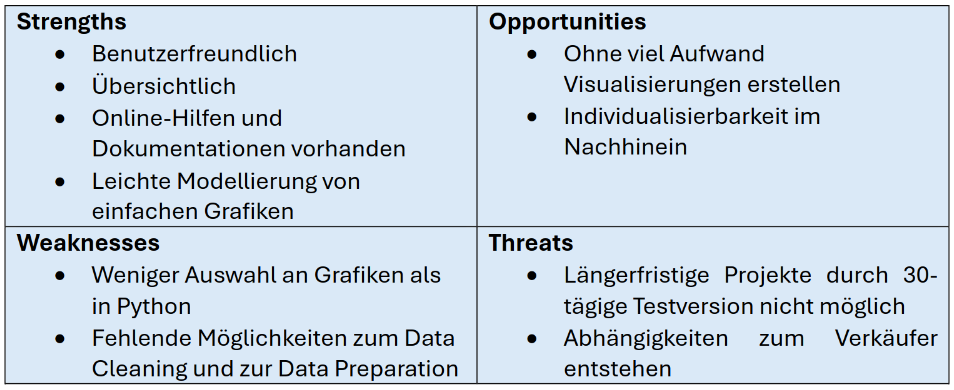
\includegraphics[width=0.5\textwidth]{SWOT3}
		\caption{SWOT Analyse Qlik Data Scientist}
	\end{figure}
	
	\subsubsection{Betrieblicher Entscheider}
	
	Um für den betrieblichen Entscheider auch eine Auswahl zwischen den Tools zu
	ermöglichen, wird für diesen nun auch noch eine SWOT-Analyse bezüglich Qlik erstellt.
	Für diesen ist es vermutlich eher weniger wichtig umfangreiche Datenvisualisierungen
	zu entwerfen, wie es der Data Scientist für gewöhnlich bewerkstelligt. Der betriebliche
	Entscheider verfolgt primär das Ziel, so effizient wie möglich Dashboards für die
	Entscheidungsfindung in seinem Unternehmen zu entwerfen.
	Hierfür benötigt er ein übersichtliches und benutzerfreundliches Tool, mit welchem er
	schnell und einfach passende Visualisierungen erzeugen kann. Dies erhält er mit dem
	Verwenden von Qlik, indem er auf der Startseite einen Überblick über grundlegende
	Diagrammarten erhält und diese per einfachem Mausklick auswählen kann.
	Somit kann er die Stärken des Tools sehr gut ausnutzen.
	Des Weiteren dürfte ihm zugutekommen, dass keinerlei Programmiererfahrungen
	notwendig sind, um adäquate Ergebnisse liefern zu können, wenn der importierte
	Datensatz bereits vollständig bereinigt ist. Wie dem Data Scientist, können hierbei auch
	die zahlreichen Dokumentationen im Internet dem betrieblichen Entscheider dabei
	helfen, bei Unklarheiten voranzukommen.
	Nachteile bieten ihm sich nur dann, wenn er versucht mit einem Datensatz zu arbeiten,
	der Inkonsistenzen enthält. Dadurch könnten seine Visualisierungen dann unbrauchbar
	werden, da zu viele Fehlstellen in die erstellte Grafik eingebaut werden.
	Ebenfalls könnte auch für ihn die teure Vollversion des Tools zum Problem werden, wenn
	das Geld für dieses nicht vorhanden ist. Wobei die finanzielle Sachlage im betrieblichen
	Kontext weniger ein Problem sein dürfte als beim Data Scientist, der das Tool auch für
	private Zwecke benutzt.
	\begin{figure}[h]
		\centering
		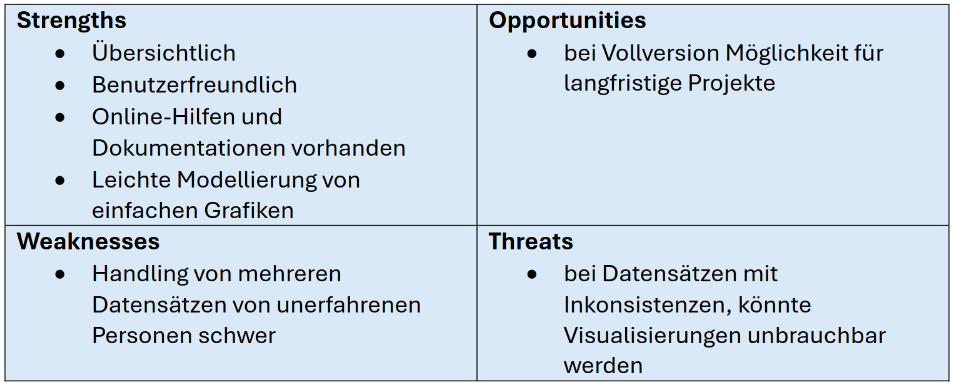
\includegraphics[width=0.5\textwidth]{SWOT4}
		\caption{SWOT Analyse Qlik Betrieblicher Entscheider}
	\end{figure}
	
	\section{Fazit}
	
	Da in der heutigen Gesellschaft, sowohl im privaten als auch betrieblichen Umfeld,
	Daten eine immer größere Rolle spielen, ist es wichtig auch ein geeignetes Tool für den
	jeweiligen Anwendungszweck zu ermitteln.
	Deshalb wurde die Analyse von Python und Qlik und deren Vergleich in der Ausarbeitung
	zum zentralen Bestandteil.
	Als abschließendes Fazit zu jener Toolanalyse, kann festgehalten werden, dass beide
	Tools für jeweilige spezifische Anwendungsfälle ihre Vor- und Nachteile besitzen.
	Python hat sich im Laufe der Analyse als Tool herausgestellt, in welchem die
	Möglichkeiten zur Datenvisualisierung durch den Einsatz verschiedener Bibliotheken wie
	Plotly oder Pandas nahezu unbegrenzt sind.
	Mannigfaltige Varianten an Modellierungsarten können hierfür ausgewählt werden.
	Sind die nötigen Programmiererfahrungen beim jeweiligen Endanwender vorhanden, so
	kann mit umfangreichen Datenmengen gearbeitet und durch die Möglichkeit von
	Datenbereinigung und Datenvorbereitung, für die letztendliche Verwendung, auch ein
	präzises Visualisierungsergebnis erzielt werden.
	Mögliche Anwendungsszenarien für Python könnten, aufgrund der freien Verfügbarkeit
	ohne zusätzliche Kosten, die Privatanwendung bei Personen, die sich schlichtweg für
	den Umgang mit Daten interessieren, aber auch die Nutzung in Unternehmen sein.
	Gerade im unternehmerischen Kontext, in welchem tagtäglich mit großen Datenmengen
	gearbeitet wird, benötigt es ein flexibel einsetzbares Tool, das weitreichende Ergebnisse
	in Bezug auf Daten liefern kann. Dafür ist Python auf jeden Fall sehr gut geeignet, da
	Unternehmen auch meistens Mitarbeiter beschäftigen, die genau auf solche
	Anwendungsfälle spezialisiert sind und das nötige Hintergrundwissen besitzen, um die
	verschiedenen Befehle und Bibliotheken einzusetzen.
	Als Vergleichsobjekt zu Python wurde auch Qlik analysiert. Das cloudbasierte Tool
	zeichnet sich vor allem durch seine übersichtliche Oberfläche, in welcher leichte
	Visualisierungen ohne geringen Aufwand erstellt und auch individualisiert werden
	können, aus. Im Gegensatz zu Python bedarf es hierbei keinerlei Erfahrung im Umgang
	mit Programmiersprachen, sodass praktisch jeder es benutzen kann.
	Allerdings stellen die hohen monatlichen Kosten eine Barriere für die Nutzung von
	Privatpersonen dar. In dieser Hinsicht kann Python mit umfassenderen Möglichkeiten im
	Umgang mit Daten bevorzugt werden. Vor allem als Data Scientist außerhalb des
	Geschäfts-betrieblichen Prozesses, ergeben sich aus dem leichten Erstellen für
	einfache Visualisierungen kaum Vorteile, welche die monatliche Bezahlung von 30 US-
	Dollar rechtfertigen.
	Trotzdem ist Qlik für den betrieblichen Kontext eine Option, in welchem es ein
	Anwendungsszenario finden kann.
	Ein Beispiel hierfür könnte ein Angestellter sein, welcher keine Programmiererfahrung
	besitzt, aber dennoch einfache Visualisierungen für eine Präsentation konzipieren
	möchte. Ohne größeren Aufwand kann ein anschauliches Gesamtbild erzeugt werden,
	was seinen Zweck erfüllt.
	Da auch die Lizenzkosten für ein wirtschaftlich gut aufgestelltes Unternehmen kein
	Problem darstellen sollten, stellt dies ein mögliches Anwendungsszenario dar.
	Somit ist die Gesamtanalyse von Python und Qlik mit Blick auf verschiedenste Kriterien
	und dem Aufzeigen von verschiedenen Anwendungsszenarien abgeschlossen.
	
	\section{Quellen}
	% Struktur nach Quellenverzeichnis fehlt, Links, Beschreibungen hinzufügen, dann an den entsprechenden Textstellen kennzeichnen.
	
	\subsection{Quellen Datensätze}
	
	\begin{enumerate}
		\item \href{https://example.com}{Beispiel Webseite}
		\item \href{https://example.org}{Eine andere Beispiel Webseite}
		\item \href{https://example.org}{Eine andere Beispiel Webseite}
		\item \href{https://example.org}{Eine andere Beispiel Webseite}
		\item \href{https://example.org}{Eine andere Beispiel Webseite}
		\item \href{https://example.org}{Eine andere Beispiel Webseite}
		\item \href{https://example.org}{Eine andere Beispiel Webseite}
		\item \href{https://example.org}{Eine andere Beispiel Webseite}
		\item \href{https://example.org}{Eine andere Beispiel Webseite}
		\item \href{https://example.org}{Eine andere Beispiel Webseite}
		
		\subsection{weitere Quellen}
		\item \href{https://www.gapminder.org/}{Einige der Fragen an denen der Vergleich durchgeführt wurde wurden von hier übernommen}
		
	\end{enumerate}
	
\end{document}